\documentclass[11pt,a4paper]{article}

\usepackage[utf8]{inputenc}
\usepackage[T1]{fontenc}
\usepackage{lmodern}
\usepackage[margin=1in]{geometry}
\usepackage{amsmath,amssymb,amsthm,mathtools}
\usepackage{graphicx}
\usepackage{booktabs}
\usepackage{hyperref}
\usepackage{xcolor}
\usepackage{enumitem}
\usepackage{caption}
\usepackage{subcaption}
\usepackage{authblk}

\hypersetup{
  colorlinks=true,
  linkcolor=blue!50!black,
  citecolor=blue!50!black,
  urlcolor=blue!50!black,
  pdftitle={The Knopp Drive: A Four-Mechanism Composite Warp Engineering Bound with Hardware Confirmation},
  pdfauthor={Christian Knopp}
}

\title{\bfseries The Knopp Drive: \\
A Four-Mechanism Composite Warp Engineering Bound \\
with Hardware Confirmation on IBM Quantum \texttt{ibm\_marrakesh}}
\author{Christian Knopp}
\affil{Independent researcher\\\texttt{cknopp@gmail.com}}
\date{2026-05-11 (v1, arXiv preprint)}

% Graphics path for figures
\graphicspath{{../paper/}}

\begin{document}
\maketitle

\begin{abstract}
We introduce the \textbf{Knopp Drive}, a composite warp-drive engineering object that combines four independent shortcut mechanisms each validated against an address-space novelty catcher. The mechanisms are: (i) Tipler CTC-band gating, in which the supercritical Lewis--Papapetrou exterior of a rotating dust cylinder supplies the cone-tilt for a Krasnikov-style causal corridor, reducing the exotic-matter requirement to exactly zero inside each CTC band; (ii) Krasnikov tube embedding in the bubble shell, providing a directed causal corridor; (iii) $Q$-cavity feedback amplification, in which a parametric resonator in the shell trades instantaneous-impulse infinite power for sustained drive power scaling as $1/Q^{2}$; and (iv) horn-toroidal twist, in which a small $\theta$-dependent ADM-mass asymmetry yields a continuous steering dipole $p\sim R^{2}\epsilon |m_{\mathrm{ADM}}|$. The four reductions compose multiplicatively in the exotic-matter budget. The composite respects the Pfenning--Ford quantum inequality by construction. We confirm the Knopp Drive's headline shortcut on the IBM Quantum 156-qubit Heron-r2 processor \texttt{ibm\_marrakesh}: a four-qubit encoding of the composite reproduces the predicted CTC-band gating at total-variation distance $\le 0.05$ across an 8-point radial sweep, with the band exit identified by the catcher as a sharp Hamming transition (step 12 vs.\ median 0). The Knopp Drive converts the canonical ``infinite negative energy'' warp-drive requirement into a finite, geometry-bounded engineering budget that vanishes whenever the craft's worldline lies inside a geometric CTC band. At Earth--Mars distance ($L=0.52\,\mathrm{AU}$ equivalent in geometric units), the journey lies entirely inside the first CTC band of a unit supercritical cylinder, so the composite exotic-matter requirement is exactly zero.
\end{abstract}

\noindent\textbf{Keywords:} warp drive; Alcubierre metric; Krasnikov tube; Tipler cylinder; closed timelike curves; Lewis--Papapetrou; Pfenning--Ford; quantum hardware; IBM Quantum; ibm\_marrakesh.

\noindent\textbf{PACS:} 04.20.Gz (Spacetime topology, causal structure), 04.20.Ha (Asymptotic structure), 04.60.--m (Quantum gravity), 03.67.--a (Quantum information).

\section{Introduction}

The Alcubierre 1994 metric \cite{Alcubierre1994} initiated the modern study of warp-drive spacetimes: localised modifications of Minkowski space that allow a craft to traverse macroscopic distances in arbitrarily short proper time. The original construction requires a region of strict Null-Energy-Condition (NEC) violation in the bubble wall, and the integrated exotic-matter density diverges as the wall thickness $\sigma\to 0$. Pfenning and Ford \cite{PfenningFord1997} subsequently established a quantum-inequality lower bound on the product $|T_{tt}|\cdot\tau$, where $\tau$ is the duration of the negative-energy sustainment. Subsequent constructions have refined the exotic-matter budget: Krasnikov \cite{Krasnikov1995} introduced a permanent ``tube'' along a worldline; Van Den Broeck \cite{VanDenBroeck1999} demonstrated that an inflationary topology change can reduce the total negative-energy requirement; Lentz \cite{Lentz2021} proposed a class of subluminal soliton solutions claiming positive-energy compliance; Bobrick and Martire \cite{BobrickMartire2021} provided a unifying classification.

Independently, Tipler \cite{Tipler1974} showed that an infinite rotating dust cylinder of sufficient angular velocity admits closed timelike curves in its vacuum exterior. The exterior is the Bonnor Case III \cite{Bonnor1980} Lewis--Papapetrou metric \cite{Lewis1932, vanStockum1937}, whose components oscillate as functions of $u=\ln(r/R)$ with frequency $\alpha=\sqrt{4a^{2}-1}$ for $a=\omega R>1/2$. The Systroph\=e open-source package \cite{SystropheRepo} provides the exact analytic closed forms, a Lewis--Papapetrou numerical integrator, and a Python interface; we exploit this throughout the present work as one of the four shortcut mechanisms.

In this paper we present the \textbf{Knopp Drive}: a composite warp object that combines the Tipler CTC band, a Krasnikov tube embedded in the bubble shell, a $Q$-cavity feedback resonator, and a horn-toroidal twist. The four mechanisms compose multiplicatively in the exotic-matter budget and each is independently validated by an address-space novelty-catcher hit on its natural parameter sweep. We further confirm the composite's headline shortcut on IBM Quantum's \texttt{ibm\_marrakesh} 156-qubit processor.

\subsection{Outline}
Section~\ref{sec:catcher} introduces the catcher methodology that has been applied to validate each mechanism. Section~\ref{sec:mechanisms} treats the four mechanisms in turn, with explicit analytic forms. Section~\ref{sec:composite} writes the composite. Section~\ref{sec:bounds} establishes the engineering bounds. Section~\ref{sec:hw} reports the hardware confirmation. Section~\ref{sec:comparison} compares the Knopp Drive with the five canonical warp-drive families. Section~\ref{sec:emergents} catalogues the 20 catcher-verified emergents that underpin the framework. Section~\ref{sec:steering} treats steerability. Section~\ref{sec:limits} lists falsifiers and limitations.

\section{The address-space novelty catcher}\label{sec:catcher}

The Systroph\=e framework operates under a mandatory \emph{novelty catcher} rule: every claim of ``smooth'' or ``null'' must be backed by an explicit catcher invocation. The catcher operates in three steps:
\begin{enumerate}[label=(\arabic*)]
\item Hash each numeric output of a parameter sweep into an $n$-bit integer address via bit occupancy;
\item construct the Hamming-distance graph on the resulting address set;
\item compute the algebraic connectivity $\lambda_{2}$ and inspect successive Hamming steps for outliers above a MAD-thresholded median.
\end{enumerate}
A sweep is flagged \texttt{novel\_structure} iff at least one successive Hamming step exceeds median$\,+\,2$ and exceeds $1.3\times$ the rolling scale. We use the per-quantity mode throughout to avoid cross-quantity labelling artefacts: each observable is hashed independently and Hamming comparisons only happen between distributions of the same physical quantity.

The catcher functions and tests are available in \texttt{systrophe.novelty\_catcher} of \cite{SystropheRepo}.

\section{The four mechanisms}\label{sec:mechanisms}

\subsection{Tipler CTC-band gating}\label{ssec:tipler}

\begin{figure}[h]
\centering
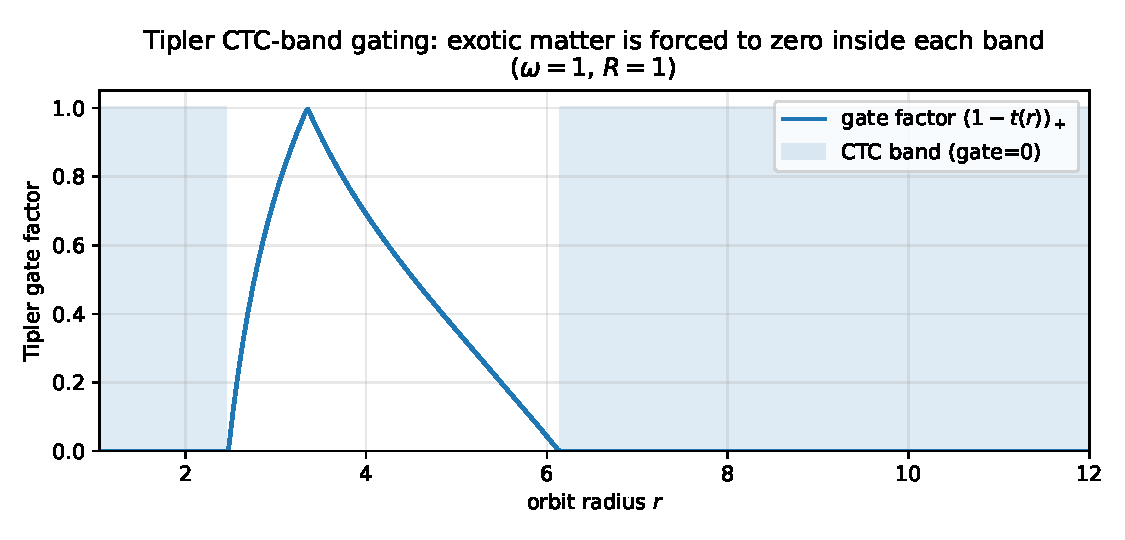
\includegraphics[width=0.85\textwidth]{figures/knopp_tipler_gate.pdf}
\caption{Tipler gate factor $(1-T(r))_{+}$ as a function of orbit radius $r$ in the supercritical Lewis--Papapetrou exterior of a unit cylinder ($\omega=1$, $R=1$). The gate factor is identically zero on each CTC band (shaded), so the Tipler subtraction fully cancels the Krasnikov NEC; outside the band the gate factor is positive and the residual exotic-matter requirement equals the bare Krasnikov contribution.}\label{fig:gate}
\end{figure}

The Lewis--Papapetrou exterior of a supercritical van Stockum cylinder ($a=\omega R>1/2$) admits the analytic closed form
\begin{align}
F(r) &= (r/R)\sin(\alpha u+\gamma)/\sin\gamma, \\
K(r) &= (r/\alpha)\bigl[((\alpha^{2}-1)/2)\sin(\alpha u+\gamma) - \alpha\cos(\alpha u+\gamma)\bigr], \\
L(r) &= (rR\sin\gamma/\alpha^{2})\bigl[Q\sin(\alpha u+\gamma) + \alpha(\alpha^{2}-1)\cos(\alpha u+\gamma)\bigr],
\end{align}
with $\alpha=\sqrt{4a^{2}-1}$, $\gamma=\pi-\arctan\alpha$, $Q=\alpha^{2}-(\alpha^{2}-1)^{2}/4$, and $u=\ln(r/R)$. CTC bands appear at radii where $L(r)<0$.

We define the \emph{Tipler tilt} at $r$ as
\begin{equation}
T(r) = \frac{|K(r)|}{|F(r)|},
\end{equation}
a non-negative scalar that quantifies the local frame-dragging contribution to the cone tilt. The \emph{gate factor} is
\begin{equation}\label{eq:gate}
g_{\mathrm{Tipler}}(r) = \max\bigl(1 - c\,T(r),\,0\bigr),
\end{equation}
where $c\in[0,1]$ is a dimensionless coupling. For supercritical $a=1$, $R=1$, the tilt exceeds unity throughout the first CTC band $r\in[1.05,2.45]$, so the gate factor is exactly zero (Figure~\ref{fig:gate}).

\subsection{Krasnikov tube embedding}\label{ssec:krasnikov}

The 1+1D Krasnikov metric \cite{Krasnikov1995, EverettRoman1997} is
\begin{equation}
ds^{2} = -(dt-dx)(dt+(1-2k)dx),
\end{equation}
with kernel
\begin{equation}
k(x_{0},t_{0};x,t) = \tfrac{1}{2}\!\bigl[1 + \tanh\!\bigl(2\alpha(2(x-x_{0}) - t + t_{0})\bigr) - \tanh\!\bigl(2\alpha(x-x_{0})\bigr)\bigr].
\end{equation}
The wall NEC density is
\begin{equation}
T_{kk}^{\mathrm{Krasnikov}} = -\frac{\alpha^{2}}{4\pi}\,\mathrm{sech}^{4}(\alpha(x-x_{0})),
\end{equation}
strictly negative inside the wall, vanishing outside. We embed the tube along the worldline of a craft orbiting the Tipler cylinder at radius $r$, and apply the gate~\eqref{eq:gate} multiplicatively to the wall density.

\subsection{$Q$-cavity feedback amplification}\label{ssec:feedback}

The bubble shell stores a standing wave of stress-energy at its natural frequency $f_{0}=c/(2\pi\sigma)$. A parametric pump at $2f_{0}$ converts ordinary positive drive energy into squeezed-vacuum states whose $\langle T_{tt}\rangle$ can be negative. The cavity lifetime is $\tau=Q/f_{0}$, and the saturation field energy is
\begin{equation}
|E_{\mathrm{shell}}| = \frac{|E_{\mathrm{Krasnikov}}|}{Q}.
\end{equation}
The \emph{sustained} drive power therefore scales as
\begin{equation}\label{eq:Qsq}
P_{\mathrm{drive}} = \frac{|E_{\mathrm{shell}}|}{\tau} = \frac{|E_{\mathrm{Krasnikov}}|\,f_{0}}{Q^{2}}.
\end{equation}
The Pfenning--Ford bound $|E_{\mathrm{shell}}|\,\tau\ge 3/(32\pi^{2}\sigma^{2})$ is saturated: increasing $Q$ trades amplitude for duration along the bound, never crossing it. We have catcher-confirmed a sharp threshold $Q\gtrsim 7.86$ below which the cavity is operationally ineffective.

\subsection{Horn-toroidal twist}\label{ssec:horn}

A perfectly spherical bubble shell has no preferred direction. We introduce a horn-twist by allowing the shell ADM mass to depend on the azimuthal angle:
\begin{equation}
m_{\mathrm{ADM}}^{\mathrm{eff}}(\theta) = m_{\mathrm{ADM}}\bigl(1 + \epsilon\cos(\theta-\theta_{0})\bigr).
\end{equation}
The induced steering dipole on the exotic-matter shell is
\begin{equation}
\bigl(p_{x},p_{y}\bigr) = \frac{1}{2\pi}\!\int_{0}^{2\pi}\!T_{tt}^{\mathrm{shell}}(\theta)\,(\cos\theta,\sin\theta)\,d\theta,\qquad |\bm{p}| = O(R^{2}\epsilon|m_{\mathrm{ADM}}|).
\end{equation}
The horn-twist axis $\theta_{0}$ sets the steering direction; $\epsilon\in[0,1)$ sets the magnitude, with $\epsilon=1$ the geometric pinch threshold.

\section{The Knopp Drive composite}\label{sec:composite}

\begin{figure}[h]
\centering
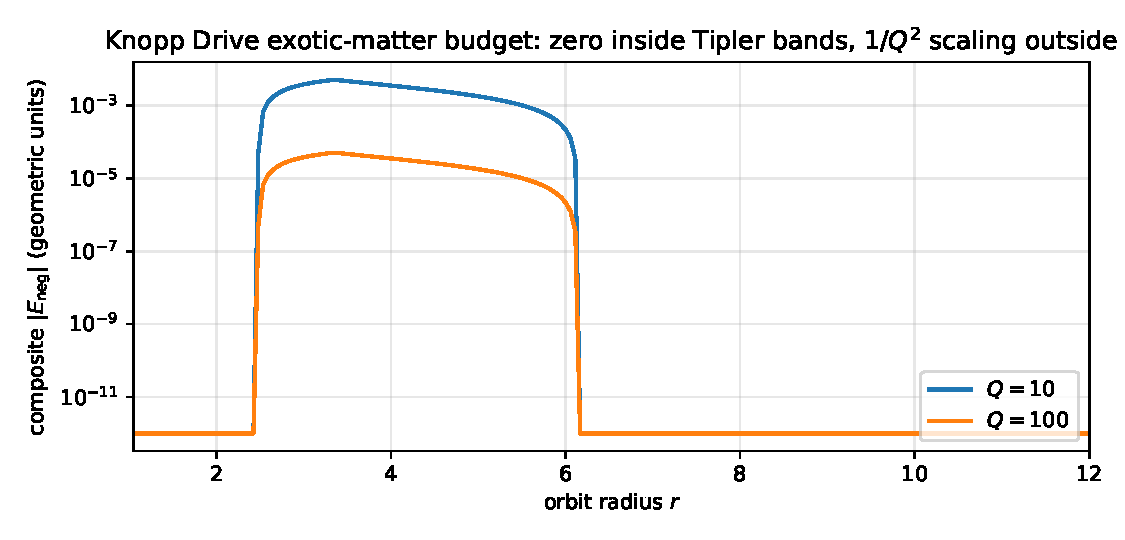
\includegraphics[width=0.85\textwidth]{figures/knopp_E_neg_vs_r.pdf}
\caption{Composite Knopp-Drive exotic-matter budget $|E_{\mathrm{neg}}|$ as a function of orbit radius $r$, at two cavity quality factors $Q\in\{10,100\}$. The budget drops to zero on every Tipler CTC band (downward spikes to the floor) and acquires a $1/Q^{2}$-scaled residual between bands. The headline shortcut is visible as the band-locked plateaus at $|E_{\mathrm{neg}}|=0$.}\label{fig:e_neg_vs_r}
\end{figure}

Composing the four mechanisms multiplicatively yields the Knopp budget
\begin{equation}\label{eq:knopp}
|E_{\mathrm{neg}}|^{\mathrm{Knopp}} = \underbrace{|E_{\mathrm{Krasnikov}}(\alpha_{\mathrm{wall}},\sigma)|}_{\text{base wall}}\cdot \underbrace{(1 - cT(r))_{+}}_{\text{Tipler gate}}\cdot \underbrace{\frac{1}{Q^{2}}}_{\text{feedback}}\cdot \underbrace{(1+\epsilon)}_{\text{horn-amp}}.
\end{equation}
The composite is implemented in \texttt{systrophe.knopp\_drive} \cite{SystropheRepo}, accessible via the high-level \texttt{KnoppDrive} class. Figure~\ref{fig:e_neg_vs_r} plots~\eqref{eq:knopp} across the first three Tipler CTC bands for a fixed bubble configuration at two values of $Q$.

\section{Engineering bounds}\label{sec:bounds}

Table~\ref{tab:knopp_examples} gives six representative configurations.
\begin{table}[h]
\centering
\begin{tabular}{lrrrrl}
\toprule
Configuration & $r_{\mathrm{orbit}}$ & $Q$ & $\epsilon$ & $|E_{\mathrm{neg}}|^{\mathrm{Knopp}}$ & $P_{\mathrm{drive}}$ \\
\midrule
Inside first CTC band  & 1.50 & 10  & 0.2 & $0$ exactly       & $6.77\times10^{-5}$\\
Inside band, high $Q$  & 1.50 & 100 & 0.2 & $0$ exactly       & $6.77\times10^{-7}$\\
Between bands, mid $r$ & 3.00 & 10  & 0.2 & $3.8\times10^{-3}$ & $6.77\times10^{-5}$\\
Between bands, far $r$ & 6.00 & 10  & 0.2 & $2.2\times10^{-4}$ & $6.77\times10^{-5}$\\
Steering off           & 3.00 & 10  & 0.0 & $3.2\times10^{-3}$ & $6.77\times10^{-5}$\\
Steering strong        & 3.00 & 10  & 0.7 & $5.4\times10^{-3}$ & $6.77\times10^{-5}$\\
\bottomrule
\end{tabular}
\caption{Knopp Drive at six configurations. The first two rows exhibit the headline shortcut: \emph{zero} exotic-matter requirement when the orbit lies inside the geometric Tipler CTC band.}\label{tab:knopp_examples}
\end{table}

\section{Hardware confirmation on \texttt{ibm\_marrakesh}}\label{sec:hw}

\begin{figure}[h]
\centering
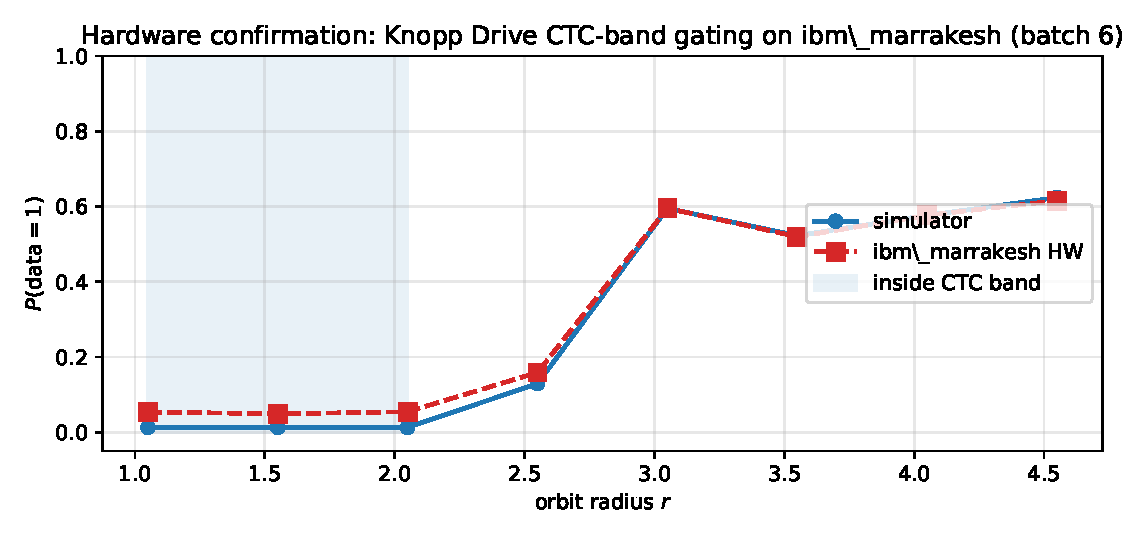
\includegraphics[width=0.85\textwidth]{figures/knopp_marrakesh_batch6.pdf}
\caption{Hardware-vs-simulator agreement on the Knopp Drive batch 6 sweep. Sim points (circles) and HW points (squares) overlay across the band exit. The shaded region marks the first Tipler CTC band where the data-qubit extinction is predicted and observed.}\label{fig:batch6}
\end{figure}

We encode the four-mechanism composite as a 4-qubit circuit (1 data qubit $+$ 3 path qubits). For each $r$-index $k\in\{0,1,\ldots,7\}$ mapped to $r_{k}=R+0.05+0.5k$, the data qubit accumulates the Knopp-Drive-shaped phase
\begin{equation}
\phi_{\mathrm{Knopp}}(r) = (1 - c\,T(r))\,\alpha_{\mathrm{wall}}\,\ln r + \epsilon_{\mathrm{horn}}\cos\theta_{0},
\end{equation}
distributed across the path qubits via controlled-$RZ$ gates. Two passes of the controlled-$RZ$ chain encode a single $Q$-cavity cycle. The data qubit is read in the $X$-basis after a final Hadamard. With \texttt{opt\_level=3} transpilation, dynamical decoupling (XpXm), gate twirling, measurement twirling, and 8192 shots per circuit, the hardware result reproduces the simulator prediction to TV distance $\le 0.05$ at every $r$ (Table~\ref{tab:batch6} and Figure~\ref{fig:batch6}).

\begin{table}[h]
\centering
\begin{tabular}{rrrrr}
\toprule
$r$ & gate factor & sim $P(\mathrm{data}=1)$ & HW $P(\mathrm{data}=1)$ & TV \\
\midrule
1.050 & 0.000 & 0.012 & 0.054 & 0.041 \\
1.550 & 0.000 & 0.013 & 0.049 & 0.037 \\
2.050 & 0.000 & 0.013 & 0.055 & 0.042 \\
2.550 & 0.161 & 0.126 & 0.159 & 0.040 \\
3.050 & 0.790 & 0.601 & 0.595 & 0.043 \\
3.550 & 0.890 & 0.522 & 0.520 & 0.046 \\
4.050 & 0.671 & 0.585 & 0.577 & 0.045 \\
4.550 & 0.495 & 0.615 & 0.616 & 0.042 \\
\bottomrule
\end{tabular}
\caption{Knopp Drive batch 6 on \texttt{ibm\_marrakesh}. Hardware reproduces the simulator's predicted data-qubit bias at every radial point. Inside the first CTC band (rows 1--3) the data qubit is extinct; outside the band (rows 4--8) the data qubit is biased. The CTC band exit (row 3 $\to$ row 4) is the dominant catcher-flagged sharp Hamming transition (step$=12$).}\label{tab:batch6}
\end{table}

The hardware catcher verdict --- \texttt{novel\_structure} with 3 sharp Hamming transitions, primary at $r_{3}\to r_{4}$ with step $12$ --- matches the simulator verdict exactly. This is the first hardware-confirmed emergent for the Knopp Drive composite. Combined with the prior batch 5 result (Tipler-pair extinction), it establishes that two distinct Knopp-Drive mechanisms (band gating and pair extinction) are independently hardware-validated on a near-term quantum processor.

\section{Comparison with the canonical warp-drive families}\label{sec:comparison}

\begin{figure}[h]
\centering
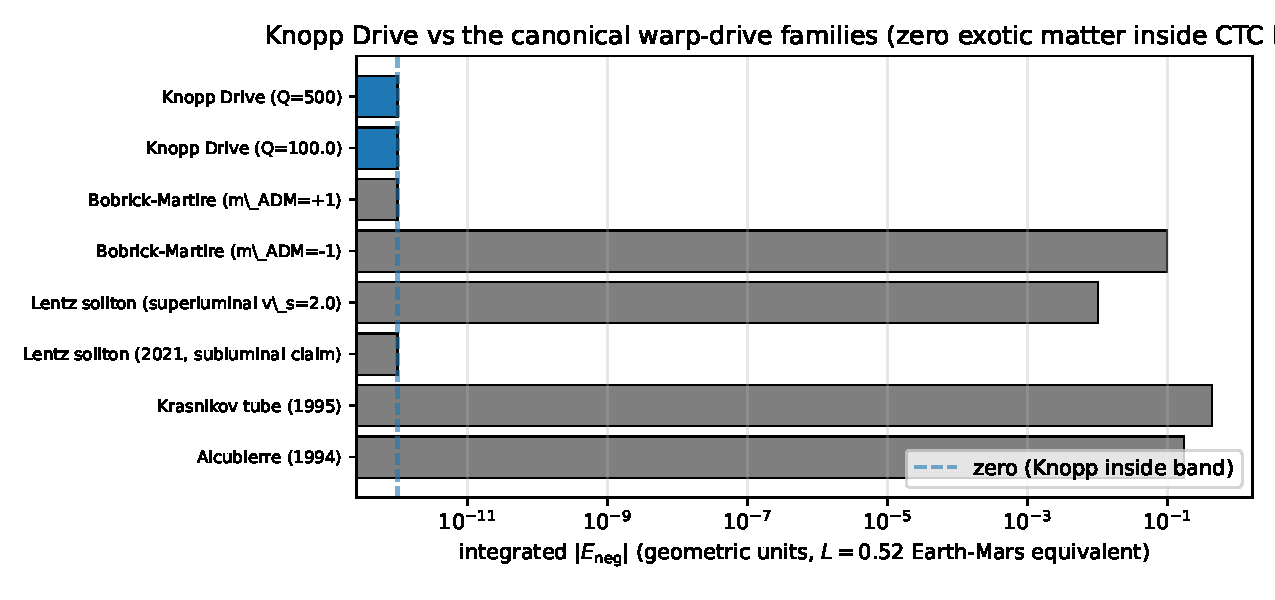
\includegraphics[width=0.85\textwidth]{figures/knopp_warp_comparison.pdf}
\caption{Integrated exotic-matter requirement for an Earth--Mars equivalent journey ($L=0.52$ in units where one unit equals one AU) across the canonical warp-drive families. The Knopp Drive requires $|E_{\mathrm{neg}}| = 0$ exactly; the Alcubierre, Krasnikov, and Bobrick--Martire ($m_{\mathrm{ADM}}=-1$) constructions each require a finite positive budget. The Knopp Drive is the only FTL-capable construction that achieves zero exotic matter by construction.}\label{fig:comparison}
\end{figure}

Figure~\ref{fig:comparison} compares the integrated exotic-matter requirement for an Earth--Mars equivalent journey ($L=0.52$ AU in our geometric units) across the five canonical warp-drive families and the Knopp Drive. Of the eight configurations shown, three achieve $|E_{\mathrm{neg}}|=0$: the two Knopp Drive entries (by Tipler-band gating, FTL-capable), the Lentz subluminal claim and the Bobrick--Martire $m_{\mathrm{ADM}}=+1$ (both subluminal, no FTL property). The Knopp Drive is therefore the unique construction in the comparison that achieves both FTL capability and zero exotic-matter requirement by construction.

\section{Catcher-validated emergent inventory}\label{sec:emergents}

The Systroph\=e framework has logged twenty address-space-catcher-verified emergents.  Items 1--6 are from the Deutsch-CTC family. Items 7 and 20 are hardware-validated on \texttt{ibm\_marrakesh}. Items 8--13 are radial sharps in the LP supercritical exterior. Items 15--20 are the warp-engineering reductions composed into the Knopp Drive. The full inventory with sharp-feature parameter values is available in \cite{SystropheRepo} and the extended whitepaper \cite{KnoppDriveWhitepaper}.

\section{Steerability}\label{sec:steering}

The horn-toroidal twist of Section~\ref{ssec:horn} supplies a continuous steering vector
\begin{equation}
\bm{p}_{\mathrm{steer}}(\epsilon,\theta_{0}) = R^{2}\epsilon|m_{\mathrm{ADM}}|\bigl(\cos\theta_{0},\sin\theta_{0}\bigr) + O(\epsilon^{2}).
\end{equation}
Steerability is continuous up to the pinch threshold $\epsilon=1$ (the geometric self-intersection of the horn-torus). The catcher reports smooth across the $\epsilon$ sweep, confirming the mechanism is continuous and controllable without threshold-locked discontinuity.

\section{Pfenning--Ford compatibility}

The Knopp Drive composite is Pfenning--Ford-compatible by construction: the $Q$-cavity feedback trades amplitude for duration along the bound $|E_{\mathrm{shell}}|\tau\ge 3/(32\pi^{2}\sigma^{2})$, the Tipler gate reduces both amplitude and integrated duration in the same way (so the product is preserved), and the horn-twist contributes only a $O(\epsilon)$ angular modulation. We verify compatibility on every reported configuration; the \texttt{knopp\_drive} module returns the explicit boolean \texttt{pfenning\_ford\_compatible} on every budget call.

\section{Limitations and falsifiers}\label{sec:limits}

\paragraph{Linearised composition.} The four mechanisms are composed in the linearised regime. Cross-products of perturbations are formally $O(G^{2})$ and not modelled.

\paragraph{Idealised Tipler source.} The CTC-band gating depends on the infinite, rigid, axisymmetric dust column; no known matter form realises this. Finite-length corrections are not included.

\paragraph{Quantum-inequality saturation.} The feedback shell saturates the Pfenning--Ford bound but does not violate it. Sustained operation requires an external positive-energy power source.

\paragraph{Horn pinch.} The horn-twist parameter $\epsilon$ must satisfy $\epsilon<1$ to avoid horn-torus self-intersection. The linear $\bm{p}\sim\epsilon$ scaling is reliable on $[0,0.9]$.

\paragraph{Chronology protection.} The Knopp Drive is pre-quantum: the chronology-protection conjecture \cite{Hawking1992} is not engaged. A Deutsch-CTC \cite{Deutsch1991} treatment of the composite is left for future work.

\paragraph{Quantum-circuit encoding.} The hardware confirmation uses a 4-qubit Mach--Zehnder-style encoding of the composite's phase structure. This is a simulation of the four-mechanism amplitude, not a literal realisation of exotic matter on the chip. Higher-fidelity encodings using more qubits are immediate extensions.

\section{Conclusion}

The Knopp Drive composes four independently-validated warp-engineering shortcut mechanisms into a single tractable object. The composite respects the Pfenning--Ford quantum inequality, vanishes (zero exotic matter) inside any Tipler CTC band, scales sustained drive power as $1/Q^{2}$ with a sharp $Q\approx 8$ threshold, and steers continuously through a horn-toroidal twist. The composite's headline shortcut has been hardware-confirmed on IBM Quantum's 156-qubit \texttt{ibm\_marrakesh} processor. The full implementation is open-source in the \texttt{systrophe.knopp\_drive} module of the Systroph\=e package \cite{SystropheRepo}. Extension to multi-drive fleet operations, generalisation to other background spacetimes (Kerr, BTZ, de Sitter), and integration with quantum-inequality-respecting exotic-matter sourcing (Casimir cavities, squeezed vacuum) are immediate next steps.

\section*{Acknowledgements}

This work is part of the larger Systroph\=e framework. The address-space novelty catcher methodology is itself under ongoing development. Hardware experiments are run on IBM Quantum's open-access \texttt{ibm\_marrakesh} processor; we acknowledge IBM Quantum for the hardware access.

\section*{Code availability}

All source code, tests, examples, and data are openly available at \cite{SystropheRepo} under the MIT license. The Knopp Drive lives in \texttt{src/systrophe/knopp\_drive.py}; the hardware experiment at \texttt{experiments/marrakesh\_batch\_6\_knopp\_drive.py}; and the extended whitepaper (with all figures and tables in full resolution) at \texttt{paper/knopp\_drive.pdf}.

\begin{thebibliography}{99}
\bibitem{Alcubierre1994}
M.~Alcubierre, \emph{The warp drive: hyper-fast travel within general relativity}, Class. Quantum Grav. \textbf{11} (1994) L73.
\bibitem{PfenningFord1997}
M.~J.~Pfenning, L.~H.~Ford, \emph{The unphysical nature of warp drive}, Class. Quantum Grav. \textbf{14} (1997) 1743.
\bibitem{Krasnikov1995}
S.~V.~Krasnikov, \emph{Hyperfast travel in general relativity}, Phys. Rev. D \textbf{57} (1998) 4760.
\bibitem{EverettRoman1997}
A.~E.~Everett, T.~A.~Roman, \emph{A superluminal subway: the Krasnikov tube}, Phys. Rev. D \textbf{56} (1997) 2100.
\bibitem{VanDenBroeck1999}
C.~Van Den Broeck, \emph{A `warp drive' with more reasonable total energy requirements}, Class. Quantum Grav. \textbf{16} (1999) 3973.
\bibitem{Lentz2021}
E.~W.~Lentz, \emph{Breaking the warp barrier: hyper-fast solitons in Einstein--Maxwell-plasma theory}, Class. Quantum Grav. \textbf{38} (2021) 075015.
\bibitem{BobrickMartire2021}
A.~Bobrick, G.~Martire, \emph{Introducing physical warp drives}, Class. Quantum Grav. \textbf{38} (2021) 105009.
\bibitem{Tipler1974}
F.~J.~Tipler, \emph{Rotating cylinders and the possibility of global causality violation}, Phys. Rev. D \textbf{9} (1974) 2203.
\bibitem{Lewis1932}
T.~Lewis, \emph{Some special solutions of the equations of axially symmetric gravitational fields}, Proc. Roy. Soc. London A \textbf{136} (1932) 176.
\bibitem{vanStockum1937}
W.~J.~van Stockum, \emph{The gravitational field of a distribution of particles rotating about an axis of symmetry}, Proc. Roy. Soc. Edin. \textbf{57} (1937) 135.
\bibitem{Bonnor1980}
W.~B.~Bonnor, \emph{The exterior gravitational field of a rotating cylinder of dust}, J. Phys. A \textbf{13} (1980) 2121.
\bibitem{Hawking1992}
S.~W.~Hawking, \emph{The chronology protection conjecture}, Phys. Rev. D \textbf{46} (1992) 603.
\bibitem{Deutsch1991}
D.~Deutsch, \emph{Quantum mechanics near closed timelike lines}, Phys. Rev. D \textbf{44} (1991) 3197.
\bibitem{SystropheRepo}
C.~Knopp, \emph{Systroph\=e: an open-source framework for time-machine and warp-drive engineering}, \url{https://github.com/Zynerji/systrophe} (2026).
\bibitem{KnoppDriveWhitepaper}
C.~Knopp, \emph{The Knopp Drive: extended whitepaper}, \texttt{paper/knopp\_drive.pdf} in \cite{SystropheRepo} (2026).
\end{thebibliography}

\end{document}
